\documentclass[10pt,a4paper]{article}
\usepackage[latin1]{inputenc}
\usepackage[english]{babel}
\usepackage{amsmath}
\usepackage{amsfonts}
\usepackage{amssymb}
\usepackage{graphicx}
\usepackage{listings}
\usepackage{wrapfig}
\usepackage{url}
\usepackage{ftnxtra}
\usepackage{fnpos}
\PassOptionsToPackage{%
%backend=biber, % Instead of bibtex
backend=bibtex8,bibencoding=ascii,%
language=auto,%
style=numeric,%
%style=authoryear-comp, % Author 1999, 2010
bibstyle=alphabetic, % dashed: substitute rep. author with ---
sorting=nyt, % name, year, title
maxbibnames=10, % default: 3, et al.
%backref=true,%
natbib=true % natbib compatibility mode (\citep and \citet still work)
}{biblatex}
\usepackage{biblatex}
\usepackage{placeins}
\usepackage{hyperref}

\author{Sascha Wernegger}
\title{Keypoint based Image Retrieval under ISO Still Image Compression Standards}

\addbibresource{paper.bib} 
\begin{document}
\maketitle

\begin{abstract}
Content-based image retrieval allows search for pictures in large image databases without keyword or text annotations. Keypoints are locations of interest in the image that  are calculated from (uncompressed) pixel data of the image. In this paper, we examine the influence of image compression on image retrieval using keypoint based matching approaches. The question here is how the compression is affecting the keypoints and their descriptors, and how the matching performance is influenced by the compression ratio. Therefore the performance of the retrieval is measured in a benchmark with a database, which is compressed to the different compression formats with different compression ratios. \\
We will investigate how the number of detected keypoints and the performance is related to the compression ratio. JPEG, JPEG-2000 and JPEG-XR are the different compression techniques compared, %to see if one of them is more suitable for image retrieval tasks.
We will also show how different keypoint detection algorithms like SIFT, SURF, PHOW and ORB can cope with the compression. We will see that much of the bandwith can be reduced without influencing the matching performance that much.
\end{abstract}

\section{Introduction} 
Content-based image retrieval (CBIR) deals with the problem of searching for digital images in large databases. ''Content-based'' means that rather than using metadata, such as tags, the content of the image itself is used to find the images in the database. Typically the system is provided with a query image and has to find similar images in the database. Content based image retrieval is becoming more and more important, because of the availability of huge amounts of digital imagery. Due to limited resources such as disk space and bandwith, virtually all images are stored in compressed form. Commonly irreversible compression is used, meaning that the original image cannot be reconstructed perfectly. Such compression algorithms may produce compressed images of different quality and therefor introduce a different amount of information loss. The effect of compression may have an important influence on performance of retrieval systems in such cases.\\
Many different approaches exist to CBIR, one of them is based on keypoints that are obtained from the pixel data. Keypoints describe interest points and also their local neighborhood in the image. One of these keypoints is SIFT, and as investigated by Elhoseiny et al. \autocite{sift_jpg} the JPEG compression, has a huge impact on the bandwith, but not affects the performance of the retrieval that much. This raises the question if other compression methods perform better, or other keypoint detectors may be more robust when affected by these compressions. So JPEG, JPEG-2000 and JPEG-XR were chosen as compression formats, and the matching performance of SIFT\citep{lowe_sift}, SURF\cite{surf}, PHOW\citep{phow} and ORB\citep{orb} were observed under various compression ratios. Therefore they are tested with a retrieval benchmark using the different algorithms for keypoint detection and compressed the dataset to different formats and compression ratios.

\section{Keypoint-based image retrieval}
In the following we describe the basic approach for image retrieval using keypoints. The task of the retrieval system is to find images in a database which are similar to a given query image. The system presents its solution by presenting a list with the images retrieved and ranked for their similarity. To achieve such a matching, we can use keypoints. The basic matching framework of keypoint based approaches can be divided into extraction, description and matching.

\begin{itemize}
	\item \textbf{Extraction}\\
Extraction is the process of finding pixels that have a significant and distinct appearance. Commonly they are obtained from corners \autocite{harris_corner, fast1}, local extrema of scale space \autocite{lowe_sift}, or blob regions \autocite{donoser2006mser}.
	\item \textbf{Description}\\
Here a descriptor is computed to describe the feature of the image. The local neighborhood of the keypoint is used to calculate the descriptor, which often represents a histogram of gradients of a scaled and rotated region of the neigborhood. The descriptor is commonly either a vector \autocite{lowe_sift,surf} or a binary string \cite{calonder2010brief,orb} of a certain size and is used for comparison.
	\item \textbf{Matching}\\
To match keypoints between an input and an a reference image, the corresponding descriptors of the input are compared to all the reference descriptors in the database. In the simplest case this is basically done by searching the k-nearest neighbors using the euclidean distance. For large feature vectors and a large database such a full search over the entire database may take very long. Instead tree based searching is used to approximate k-nearest neighbor searching \autocite{arya_search}. If the descriptor is represented as binary string, a full search with a hamming distance is performed \autocite{calonder2010brief}. 
\end{itemize}

\section{Retrieval Benchmark}
The VLFeatBenchmatk software for provides a simple to use retrieval benchmark tool. It also comes with some implementations of keypoint detectors and a dataset with annotated groundtruth files for the image. Some modifications had to be made to be able to run it with our data. 
\begin{itemize}
	\item \textbf{JPEG-2000 and JPEG-XR support}\\
VLBenchmark expects the database to contain JPEG files. In order to be able to perform the keypoint detecton the images have to be read from disk, therefore they have to be decompressed and there is no built in method to decompress JPEG-2000 and JPEG-XR. So we had to provide algorithms to be able to work with these formats. We take a closer look at the compression software used in \autoref{sec:compression}
	\item \textbf{Aditional keypoint detectors}\\
To be able to compare more detection algorithms, OpenCV 3.1 was integrated to the benchmark, therefore the keypoints and descriptors had to be converted. As additional descriptors we chose ORB and SURF.
	\item \textbf{Matching of binary strings}\\
Since there are no binary descriptors used by VLFeat, no appropriate matching algorithm is available. Here OpenCV also was used to add a matching based on hamming distance, so we are able to match the descriptors of the ORB detector.	
\end{itemize}
 The retrieval benchmark closely follows the work of Jegou et. al \autocite{inria}. First the keypoints are detected, then the descriptors are extracted and matched. Now we have a the k closest matching neighbors for every of the query images descriptors. The next step is to perform a voting, where each matching database descriptor votes for the image with a specific voting scheme.
\paragraph{Voting Scheme}
A simple voting scheme is the \textit{majority voting}, where every of the k-nearest neighbors has a single vote. The matching score is the number of votes an image received. The result of the matching process is a list ordered descending by their matching score.\\
The actual voting scheme used is the \textit{query adaptive criterion} For a fixed reference rank $r \leq k$ a query descriptor query descriptor x and a descriptor y of the database, it is defined by $$\delta_r(x,y) = max(d(x,N_r(x))-d(x,y),0)$$ where $d (x;N_r(x))$ is the distance between the query descriptor x and its $r$-th NN match. So here the vote also exploits the position of the descriptor in the kNN-ranking and the distance to neighbors. Now in both cases we end up with a ranking of the images that are considered as relevant.
\paragraph{Performance Measure}
Next a performance measure is calculated. A proposed performance measure for such a retrieval system is the mean average precision(MAP) as described in \cite{philbin}. If we look at the result of the retrieval task, we may find images that not contain the image (false positives), images that are retrieved correctly(true positives), images that are correctly not retrieved (true negatives) and images that contain the object but are not retrieved (false negatives). We can calculate the precision of the result to a query as 
$$\frac{\text{true positives}}{\text{true positives+false positives}}$$
\\
But this does not consider the position of the images in the ranking, therefore we calculate the average precision. In this case we calculate the average precision $ap$  at cut-off $k$ for the individual images.
$$ap=\sum_{k=1}^n P(k)/min(m,n)$$
Where $P(k)$ is the ratio of number of relevant images followed, up to the position k, over the number k and m is the number of relevant images in the database. So the query average precision for a query simply is the average of the precision values from each relevant document in the query. And the MAP for all queries is simply the average of the average precision of the individual queries
$$MAP = \sum_{i=1}^Nap_i/N$$
where $N$ is the number of queries and $ap_i$ is the average precision of query.
\paragraph{Dataset}
One thing we did not discuss is the fact, that in order to calculate the mean average precision, we have to know the ''groundtruth'' for the query. The groundtruth of the query defines a query image and the corresponding matches contained in the database. The Oxford Building Dataset consists of 5062 images of different landmarks in Oxford collected from \textit{flickr}. The ground-truth files are also provided for 55 queries. For every query we need four files. One that defines the query image, so it clearly contains the object, and a bounding box that indicates the location of the object in the image. For every query there are also four sets of images specified.
\begin{itemize}
	\item \textbf{Good}  A nice, clear picture of the object/building.
	\item \textbf{Ok} More than 25\% of the object is clearly visible. 
	\item \textbf{Junk} Less than 25\% of the object is visible, or there are very high levels of occlusion or distortion. 
	\item \textbf{Bad} The object is not present. 
\end{itemize}
Good, Ok and Junk-images are specified in the ground truth, Bad images are images that are not specified in of any of the queries, so they definitely not contain the object.
\begin{figure}
	\includegraphics[width=0.4\textwidth]{img/query_image.jpg} 
	\caption{\textbf{Query Image} The yellow rectangle indicates the bounding box of the object}
	\label{fig:query}
\end{figure}
\begin{itemize}
	\item \textbf{Good and OK} Are treated as relevant.
	\item \textbf{JUNK} If a chunk image is retrieved it does not influence the precision, since it is neither relevant nor irrelevant.
	\item \textbf{BAD} Treated as not relevant.
\end{itemize}
\autoref{fig:query} shows a sample query image and \autoref{fig:result} shows the result of an example result of the retrieval process.
\begin{figure}
	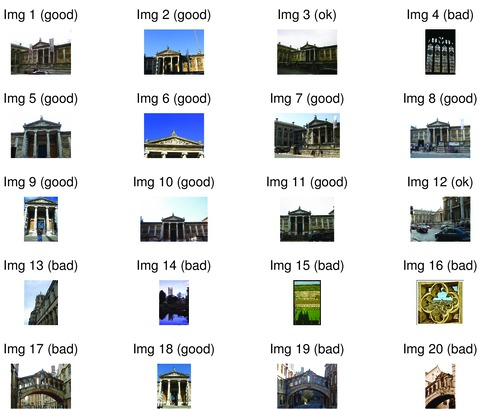
\includegraphics[width=\textwidth]{img/retrieved.jpg} 
	\caption{\textbf{Retrieved Images} Shows the top 20 images sorted by their matching score, listed from left to right an from top to bottom.}
	\label{fig:result}
\end{figure}


\FloatBarrier
\begin{wrapfigure}{r}{0.25\textwidth}
	\includegraphics[width=0.25\textwidth]{img/generation_loss.png}
	\label{fig:g_loss}
	\caption{Generation loss induced by JPEG (from top to bottom) 0, 100, 200, 500, 900, and 2000 times (without using lossless tools) \url{https://en.wikipedia.org/wiki/Generation_loss}} 
\end{wrapfigure}
\section{Compression}
\label{sec:compression}The first thing we need to mention, is the fact that the Oxford Building Dataset is already compressed in JPEG. Obtaining uncompressed datasets with an appropriate groundtruth that is not compressed is difficult due to limitations in bandwith and disk space. So sadly most data is already compressed or has no appropriate groundtruth. Therefore we have to deal with the fact that we already have some information missing. This effect is called generation loss and creates additional noise. The impact of generation loss is shown in \ref{fig:g_loss}. This effect is well known and research has been made to study the influence of it\autocite{lai2013block}.

But its influence on a retrieval task is not easy to estimate and needs more research and is needs to be considered when interpreting the data, but for now we assume the influence is minimal.\\
To run our experiment we need to compress the Oxford Buildings Dataset to different formats and different compression ratios. For each compression format we created ten compressed datasets, where we gradually increase the compression ratio to the maximum.\\
\newpage
\paragraph{JPEG} Matlab R2016b's imwrite function was used to compress to JPEG. The following quality parameters were used increase the compression ratio.
\begin{center}
	\begin{tabular}{cccccccccc}
		[0,&10,&20,&30,&40,&50,&60,&70,&80,&90]
	\end{tabular}
\end{center}
\paragraph{JPEG-2000} Her also imwrite was used, but here we have to specify the compression ratio. Choosing a to high ratio the compression fails and produces images of uniform gray pixels. From testing a maximum compression ratio from 10000 seemed to work for the database. As minimum a ratio of five was chosen resulting in the following compression ratios.
\begin{center}
	\begin{tabular}{cccccccccc}
		[5,&1116,&2226,&3337,&4447,&5558,&6668,&7779,&8889,&10000]
	\end{tabular}
\end{center}
\paragraph{JPEG-XR} For JPEG-XR we used the \textit{jxrlib} for compression because it is not supported by Matlab. The command line tool was used to generate the compressed images. Three parameters where used to achieve a gradually increasing compression ratio: \textit{Quality}, \textit{Quantization} and \textit{Chroma Sub-sampling }. Quality is used to compress the first seven datasets. The -q option may either specify the quality, which ranges from 0.0(lowest) to 1.0(lossles) or the quantization, which ranges from 1 to 255. Chroma subsampling can either be 4:4:4, 4:2:2, 4:2:0, 4:0:0 and are specified by the -d option as value from 0-3. To achieve a lower compression quantization was used instead of the quality parameter and the chroma subsampling was set to 4.0.0, meaning it considers			luminance values only. The setting for the individual values is shown below.\\
\begin{center}
	\begin{tabular}{l|cccccccccc}
		-q&[0.9,&0.8,&0.7,&0.6,&0.5,&0.4,&0.3,&50,&100,&150]\\	
		-d&[/,&/,&/,&/,&/,&/,&/,&0,&0,&0]\\
	\end{tabular}
\end{center}
\paragraph{Resulting Compression}
\ref{fig:compression} shows the file size in $mb$ for the different compression values which are also listed in the table below. 
\begin{center}
\begin{tabular}{cccccccccc}
1066.6 & 710.53 & 569.03 & 481.57 & 389.23 & 347.2 & 292.14 & 227.52 & 152.25 & 78.35
\end{tabular} 
\begin{tabular}{cccccccccc}
2135 & 10.19 & 5.27 & 3.63 & 2.81 & 2.31 & 1.98 & 1.74 & 1.56 & 1.42
\end{tabular} 
\begin{tabular}{cccccccccc}
1862.17 & 1141.4 & 857.77 & 589.65 & 470.51 & 348.12 & 259.27 & 118.89 & 28.33 & 6.83
\end{tabular} 
\end{center}
\begin{figure}[!htp]
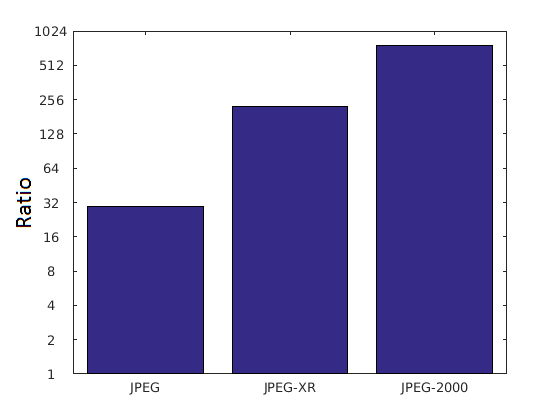
\includegraphics[width=\textwidth]{img/compression.png}
	\caption{Achieved compression ratio for the different formats}
  \label{fig:compression}
\end{figure}

\section{Results}

First we want to show the MAP for the original data set shown in fig. \ref{fig:map}.
In the next sections we will see how the detectors have performed. Therefore we show plots of the MAP over the compression ratio.

\begin{figure}[!htp]
	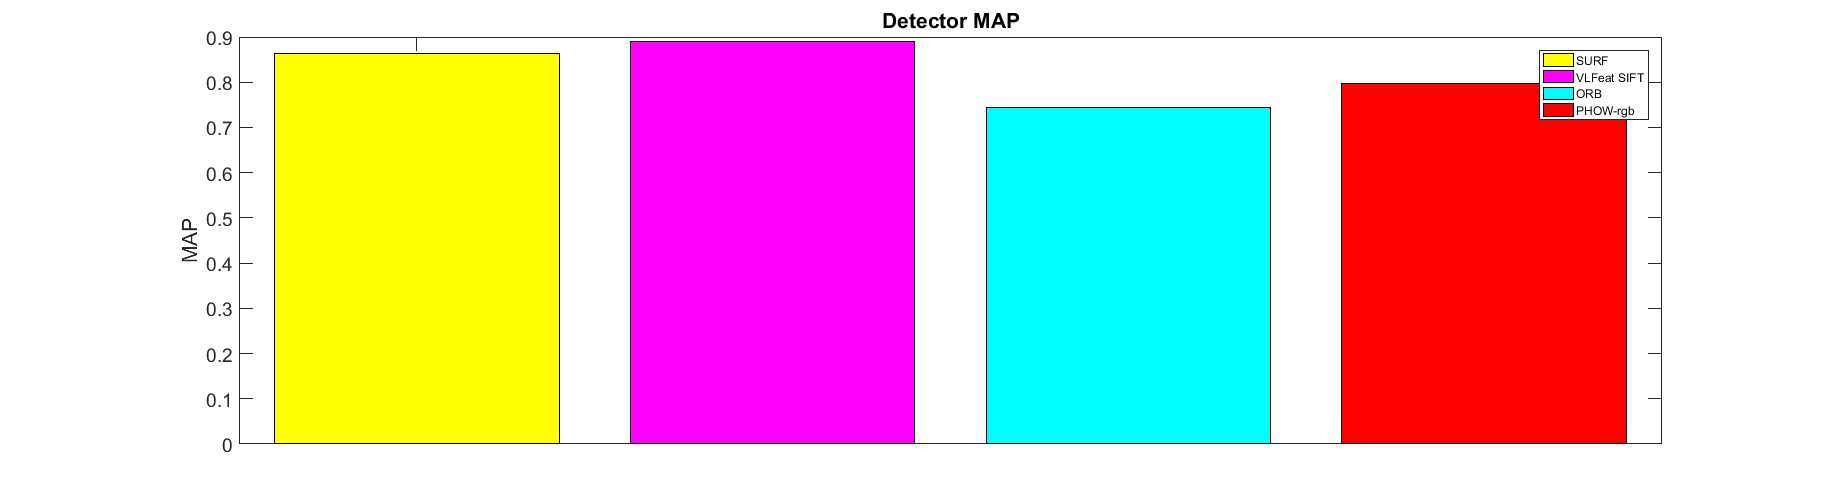
\includegraphics[width=1.2\textwidth]{img/refmap.png}
	\caption{MAP for the different descriptors on the original data set}
	\label{fig:map}
\end{figure}

For the interpretation of the results we also calculated the Mean Peak Signal to Noise Ratio (PSNR) fig. \ref{fig:psnr} for the compressed data sets, to see if there is some relation to the noise contribution.
\begin{figure}[!htp]
	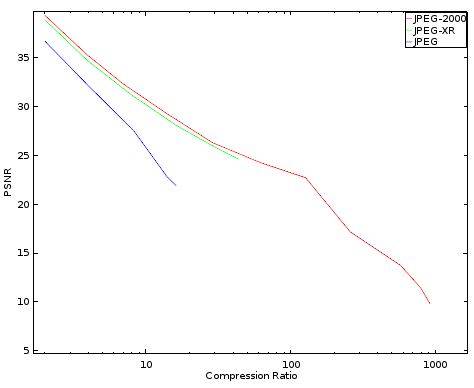
\includegraphics[width=\textwidth]{img/psnr.png}
	\caption{This shows the mean-PSNR calculated for the different compressed data
	\label{fig:psnr} sets}
\end{figure} 

\begin{figure}[!htp]
	\begin{tabular}{|c|}
		\hline \\
		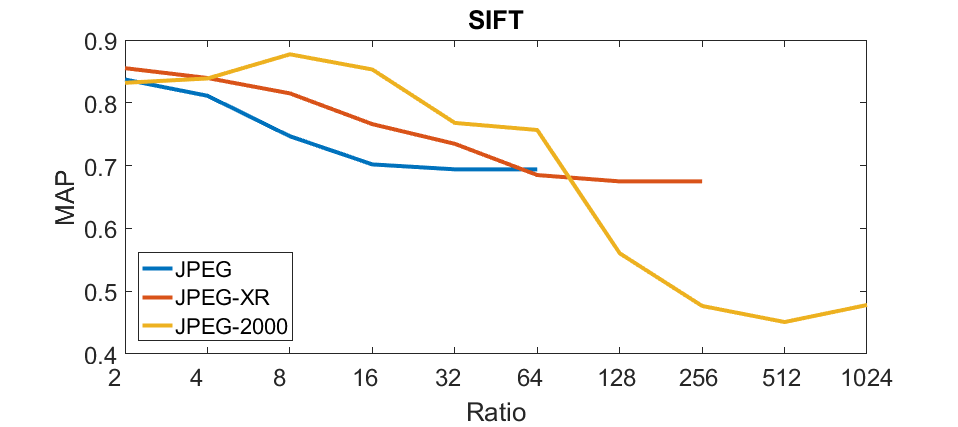
\includegraphics[width = \textwidth]{img/sift_map.png}\\
		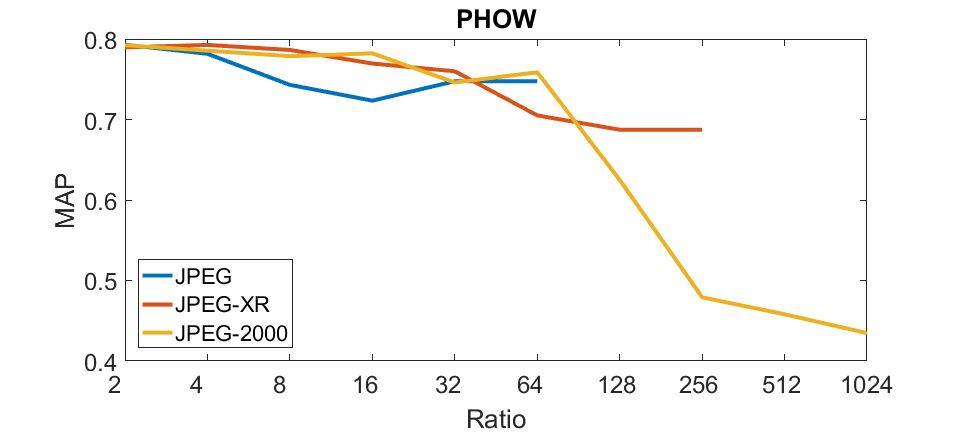
\includegraphics[width = \textwidth]{img/phow_map.png}\\
		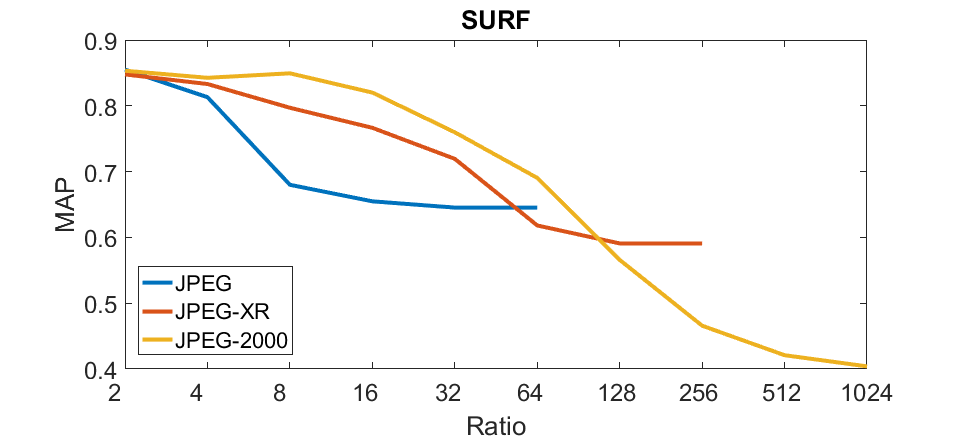
\includegraphics[width = \textwidth]{img/surf_map.png}\\
		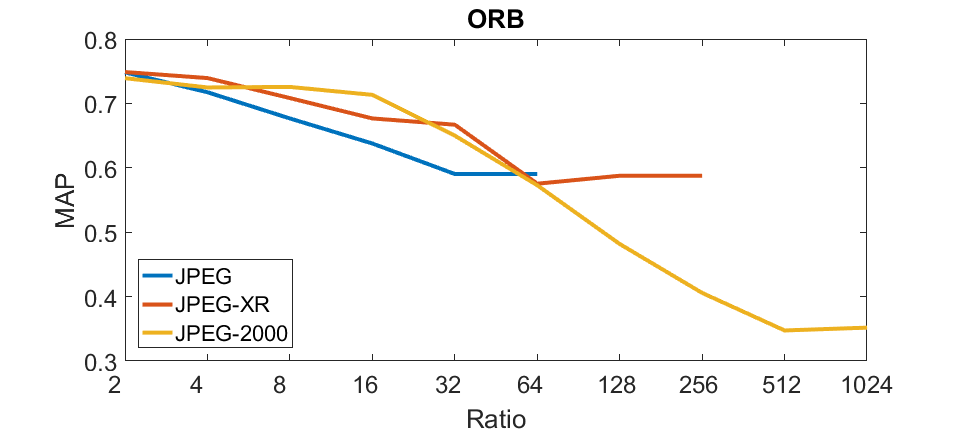
\includegraphics[width = \textwidth]{img/orb_map.png}\\
		\hline
	\end{tabular}
	\caption{plot of MAP over compression ratio for the different
	\label{fig:maps} detectors and formats}
\end{figure}
\FloatBarrier
\printbibliography
\end{document}